%---------------------------------------------------------------------------
% System tests.
%
%---------------------------------------------------------------------------
\section{System Tests}
\label{sec:tests}
\subsection{Performance tests}

In order to evaluate the system performance and to find potential bottlenecks, load tests were performed. Due to the lack of resources, the setup used for this purpose was rather simple. For test purposes I have used 2 machines: 

\begin{itemize}
\item {\bf HP nx6110} laptop having Pentium M 1.73 GHz CPU and 1.5GB of RAM, running Ubuntu Linux
\item {\bf Sony Vaio VPCEB2Z1E}, with Pentium i5 M430, running at 2.24GHz with 2 physical cores and two processing pipelines running on each core, additionally having 4GB of RAM. This machine was running Microsoft Windows7.
\end{itemize}
The above machines where connected using 100Mb Fast Ethernet switch. The test scenario was composed of following steps:

\begin{enumerate}
\item Launch Monitoring Hub Application module
\item Launch GUI module
\item On a separate machine launch 3 JVM processes that mimic a processing workflow
\item Again, on the testing machine launch \texttt{iptraf} to get insight into network load
\item Launch 2 JProfiler\footnote{\url{http://www.ej-technologies.com/products/jprofiler/overview.html}} instances, attach them to GUI and Monitoring Hub processes
\item Using GUI module and the external Monitoring Hub Application started in the previous step, add all 3 JVMs as the measured resources
\item Create 20 sample measurements, covering: Memory usage, CPU usage, per process Heap and Non Heap memory usage
\item Create 5 Visualizations, using all the types that system supports and measurements created in the previous step
\item Let the system running for a while, so it is possible to gather performance data of the system being on severe load
\item Dispose visualizations
\item Dispose measurements
\item Remove resources
\item Leave the system running for a short period of time, to make sure that CPU and memory usage returns to the values from the idle state
\end{enumerate}

In the designed scenario, I am using external Monitoring Hub Application to verify the resources usage of each component separately. Additionally, HP laptop was running a test application and Vaio was running the monitoring system. Results of tests can be found below.

Figure~\ref{fig:prof_GUI} depicts JVM telemetry measurements produced by JProfiler at the stage of tests where the system was operating under the heaviest load (Step~9 from list above). As can be seen, the system never consumed more than 90MB of used memory. The maximum of committed memory size slightly exceeded 140MB. On the other hand, the CPU time spent on the actual data processing never reached 18\%, having an average between 2\% and 8\%. What is quite interesting is the Garbage Collection, most of the time CPU time spent on garbage collection was hardly traceable, but there were 2 peaks where GC consumed nearly 20\% of CPU time. It might be cause by, so called stop-the-world garbage collection~\footnote{\url{http://en.wikipedia.org/wiki/Garbage_collection_(computer_science)#Stop-the-world_vs._incremental_vs._concurrent}}.

\begin{figure}[ht]
\centering
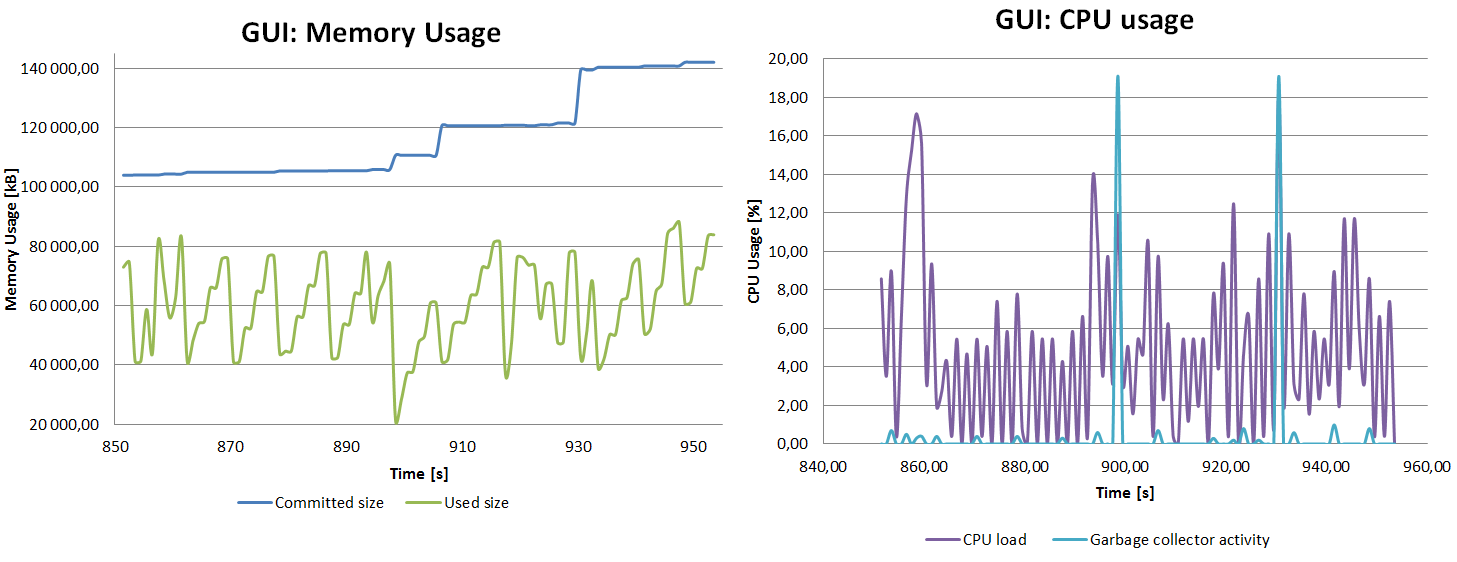
\includegraphics[width=\textwidth]{prof_GUI}
\caption{Profiling results of GUI component}
\label{fig:prof_GUI}
\end{figure}


As it is easily predictable, the Monitoring Hub module was consuming a significantly smaller portion of resources then the GUI. Figure~\ref{fig:prof_mon_hub} covers telemetry of Monitoring Hub JVM process in the same time frame (step 9 of test scenario). CPU usage of the Monitoring Hub was only a fraction of GUI usage - a peak was about 1.6\%. Regarding memory usage - Those values also were smaller than in GUI but significant - memory really used by application was staying in 10-20MB range, commit memory was nearly constant and equal to approximately 50MB.

Additionally network usage rendered by iptraf showed near constant bit rate equal to 130kbps.

\begin{figure}[ht]
\centering
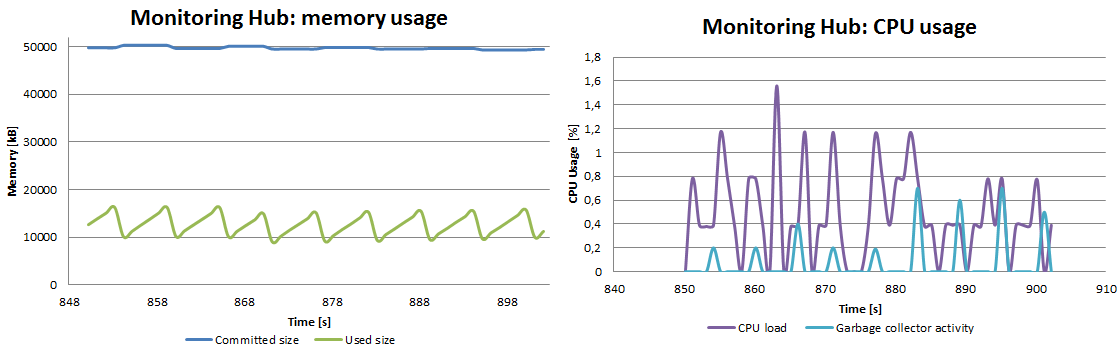
\includegraphics[width=\textwidth]{prof_mon_hub}
\caption{Profiling results of Monitoring Hub component}
\label{fig:prof_mon_hub}
\end{figure}

Test results showed clearly that performance of proposed system is good enough to say that there aren\rq{}t any significant bottlenecks, when monitoring applications of up to a medium size. Even under a severe load, the resources consumption was allowing seamless work with the application on a modern hardware. Additionally, a really low resources usage by Monitoring Hub builds solid scaffold for further scaling the application up. These results could be obtained mostly by keeping the code that is responsible for processing the measurements really simple and optimized.

\subsection{Usability tests}

As was already stated at the beginning of this chapter, in order to prove that the system is really useful, a test with real world application was performed. In this subsection, I will cover this test - from stating the sample problem, describing a solution for the problem, ending up with summary of benefits that SemSimMon gave to the work on this particular application.

Let us assume that we\rq{}ve got an assignment - create an application that will solve linear problems and that will provide a basic Web UI for accessing its services. The application should allow user to provide any square linear system using UI and will render a result vector in the same view. The application should optimize the response time rather than high throughput. Additionally, to ensure the response time, the proposed solution shall operate on an MPI-powered cluster and an external server machine that is capable of running HTTP server applications. Both cluster and HTTP server machine have the same NFS share attached. 

A solution to above the problem is a system consisting of two modules: a web application providing an interface and a processing application that solves the equations and runs on MPI cluster. The web application submits jobs to the cluster using the NFS share, by creating a request file. The solving module, checks for new jobs by polling for a new request file, solves the equation and then generates a response file. The web application, after submitting a new job file, simply waits for a solution by polling the same NFS share for a result file. 

For test purposes, solution described above was implemented. It was an application composed of 2 modules. The first one a J2EE application running on Tomcat application server, and the second one was a written in C application running on a MPI cluster. The sources of both components can be found in \texttt{test-webapp} module along with the rest of SemSimMon components.

After implementing the above application, tests under a some load were performed. Due to mentioned lack of resources, the tests were performed on cluster, composed of 2 virtual nodes. Virtual nodes were created using Oracle VirtualBox platform, and both were running 32-bit Ubuntu 9.10. The first, main node was running both HTTP server and the main node of the equation solving cluster. The second node was just computing one. For measuring the load, I have been using SemSimMon running on Guest (Windows 7) OS. 

After attaching to all resources, I have started the following metrics:

\begin{itemize}
\item A heap and a non-heap memory usage of the tomcat server
\item A CPU usage of the tomcat server
\item A system load for both MPI nodes
\end{itemize}

Figures~\ref{fig:http_cpu}~and~\ref{fig:http_memory} depicts screen shots made of the SemSimMon\rq{}s visualizations view. As we can see, the memory usage was almost constant during all the test time. The non-heap memory usage (red, labeled as HTTP NON HEAP) was between 22MB and 25MB. The heap memory usage was a bit more dynamic, but was oscillating between 3MB and 8MB. The CPU usage was traceable - between 0\% and 5.75\%. There are several areas of plots, marked with black ellipses. The areas marked with 1a and 1b in the memory usage plot and 1 in the CPU usage, points to time when I have started to sending requests the the sample application. This action caused a spike in CPU usage (1), slight increase of non heap memory (1a) and an anomaly in heap memory usage (1b). This is related to initialization of resources made by Tomcat, like compilation of JSP page into servlet. The areas marked with ellipse no 2 on both plots, represents time when system was constantly on load. As we can see, the CPU usage is in range of 0,5\% to 2,5\% and also, the garbage collection interval is a bit shorter. The ellipses labeled with 3 on both graphs shows the time frame when the system\rq{}s load test is complete and the web application is idle.

\begin{figure}[ht]
\centering
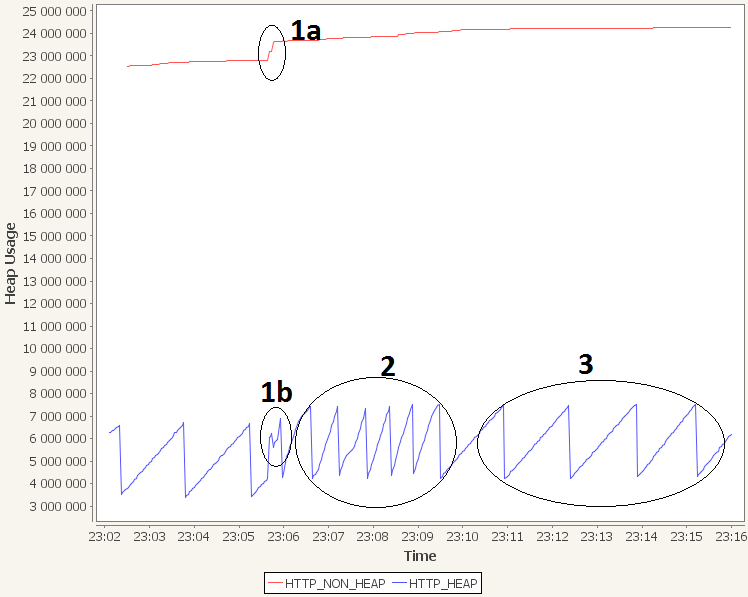
\includegraphics[width=0.7\textwidth]{memory_http2}
\caption{Test J2EE web app monitoring - memory}
\label{fig:http_memory}
\end{figure}

\begin{figure}[ht]
\centering
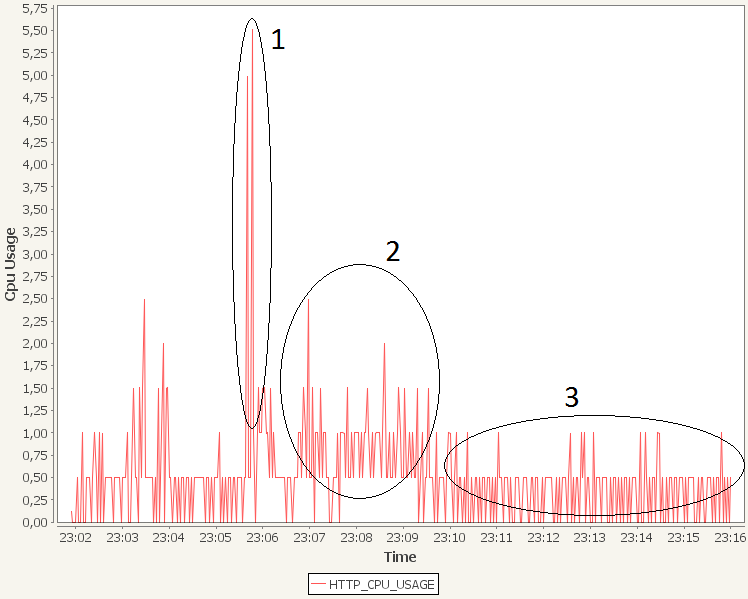
\includegraphics[width=0.7\textwidth]{CPU_USAGE_HTTP2}
\caption{Test J2EE web app monitoring - CPU}
\label{fig:http_cpu}
\end{figure}


Results of the system solver analysis are a bit more interesting. In Figure~\ref{fig:nodes_load2} we can see plot of measurement covering average load in last 1min of both nodes. The red line, labeled as \lq\lq{}CLU3 Load1\rq\rq{} represents a load of the working node (the one with rank != 0), the blue one, with the \lq\lq{}CLU1 Load1min\rq\rq{} label, represents the master node. We can see clearly that the implemented application has a huge imbalance - while the master node is mostly idle, the slave is using nearly 99\% of CPU time. The part of plot highlighted with ellipses 1a-1e represents the spikes in load due to a vast amount of jobs submitted the system. As we can see, load of master node was increasing to the level of the working nodes, but as the queue of input tasks got cleared, it was returning to almost idle state. In same time the working node was constantly using most of CPU time. Ellipse 2 and 3 shows the spike due to last testing sessions, where I have started submitting jobs after a while of a break before the 2 and between the 2 and 3. Those spikes also have a reflection in http server\rq{}s CPU usage plot. Figure~\ref{fig:load5_pie2} contains a pie chart with measurements of a Average Node Load in last 5 minutes of both those nodes. It depicts the asymmetry from a longer period of time, including the one when system was on load. Figure~\ref{fig:total_cpu_time} depicts the total CPU time of both processes running the example solver application. Here, the process running a worker routine reached 750 seconds, while the master was almost idle. This asymmetry is caused by a bug in a routines of nodes other then master - those nodes tries to received the data without any blocking in infinite loop.

\begin{figure}[ht]
\centering
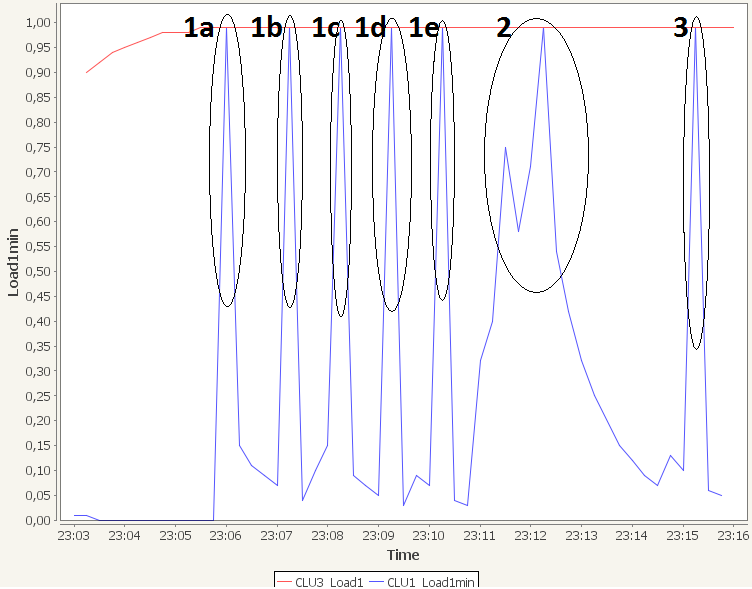
\includegraphics[width=0.8\textwidth]{nodes_load2}
\caption{MPI based linear systems solver: Node Load Average - 1min}
\label{fig:nodes_load2}
\end{figure}

\begin{figure}[ht]
\centering
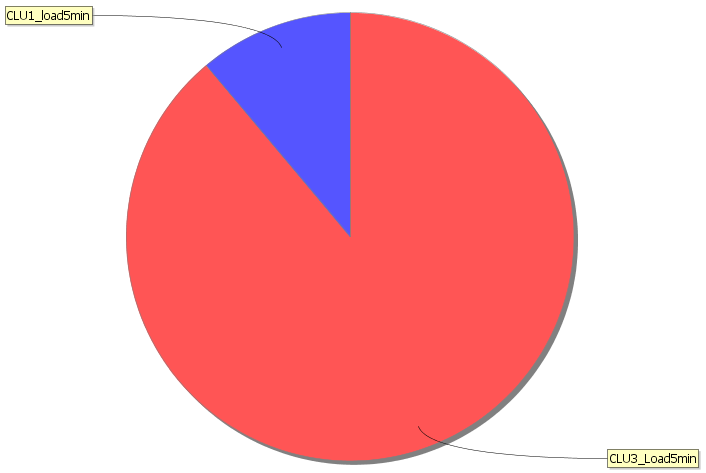
\includegraphics[width=0.5\textwidth]{load5_pie2}
\caption{MPI based linear systems solver: Node Load Average - 5min}
\label{fig:load5_pie2}
\end{figure}

\begin{figure}[ht]
\centering
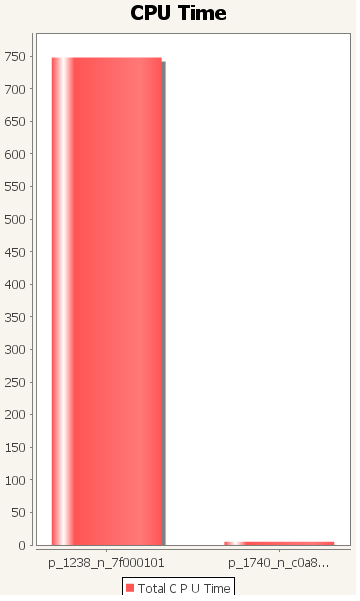
\includegraphics[width=0.4\textwidth]{cpu_time2}
\caption{MPI based linear systems solver: CPU time}
\label{fig:total_cpu_time}
\end{figure}
